\documentclass{beamer}
\usepackage[english,russian]{babel}
\usepackage[utf8]{inputenc}
\usepackage{import}
% Стиль презентации
\usetheme{Warsaw}

\beamertemplatenavigationsymbolsempty
\graphicspath{{./img/}{./img/giftWraping2D/}{./img/firstPlane/}{./img/crossP/}{./img/crossPN/}{./img/heap/}}
\usefonttheme[onlymath]{serif}
\def\svgwidth{\linewidth}
\begin{document}
\title{МНОГОМЕРНЫЙ АЛГОРИТМ ОВЫПУКЛЕНИЯ РОЯ ТОЧЕК, НАХОДЯЩИХСЯ В НЕОБЩЕМ ПОЛОЖЕНИИ}
\author[Корабельников А.А.]{\scriptsize Выполнил: студент гр. МЕНМ-280901 Корабельников А.А.\\Научный руководитель: к.ф.-м.н., доцент Кумков С.С}
\institute{Институт естественных наук и математики}
\date{Екатеринбург, 2020}
% Создание заглавной страницы
\frame{\titlepage}
% Автоматическая генерация содержания
\frame{\frametitle{Содержание}\tableofcontents}
\begin{frame}{Постановка задачи}
   Требуется разработать алгоритм построения выпуклой оболочки многомерного роя точек, находящихся в необщем положении.
   \vfill
   Необщее положение точек означает что в гиперплоскости евклидова пространства размерности $n$ лежит больше чем $n+1$ точка.\\
   \vfill
    \begin{minipage}{.49\textwidth}
    \centering
    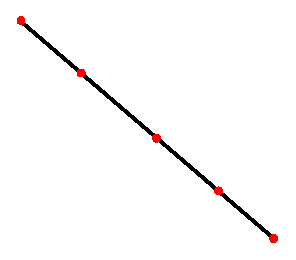
\includegraphics[width=0.5\linewidth]{line.eps}
  \end{minipage}
  \begin{minipage}{.49\textwidth}
    \centering
    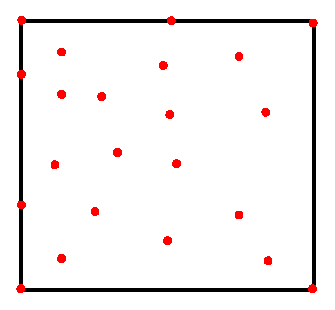
\includegraphics[width=0.5\linewidth]{cube1.eps}
  \end{minipage}
   % Пояснение в пространстве.fff
\end{frame}

\begin{frame}{Необщее положение точек}
     \begin{minipage}{.49\textwidth}
     \centering
     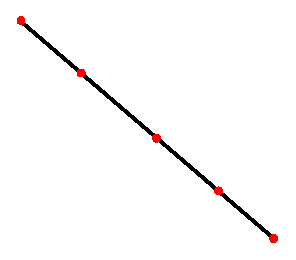
\includegraphics[width=0.8\linewidth]{line.eps}
   \end{minipage}
   \begin{minipage}{.49\textwidth}
     \centering
     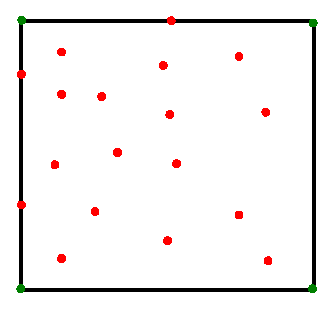
\includegraphics[width=0.8\linewidth]{cube12.eps}
   \end{minipage}

   \bigskip

   Проблемы:
   \begin{itemize}
    \item  Требуется вычислять вершины \textbf{\textit{(гипер)грани}},
    \item  Требуется вычислять \textbf{\textit{(гипер)рёбра}} грани.
    \end{itemize}
   \vfill
   Мне не известны реализации алгоритмов овыпукления, работающих в многомерном пространстве в необщем положении.
    % В многомерном пространсве эти проблемы есть, в двухмернос одни легко решаются. Объяснить сокращение.
 \end{frame}


 \begin{frame}{Алгоритмы построения выпуклой оболочки в nD}

        \vspace{0.5cm}
        % \begin{itemize}
            % \item  Quickhull - $O(n^{\left[d/2\right]})$
            % \item  Method of Clarkson and Shor  - $O(n^{\left[d/2\right]})$

            % \medskip
            % Эти два алгоритма работают в общем положении.
            % \medskip

             Многие алгоритмы для случая плоскости имеют свои аналоги в 3D, но не в большей размерности.
        % \end{itemize}
        \vspace{0.25cm}
        Библиотеки вычислительной геометрии:
        \begin{itemize}
            \item  CGAL
            \item  LEDA
        \end{itemize}
        \vfill
        \begin{center}
            \raisebox{15mm}{
            \parbox{0.3\textwidth}{Основная проблема алгоритмов, нацеленных на общее положение --- несимплициальные грани.}
            }
            \hspace{10mm}
            \includegraphics<1>[width=0.3\linewidth]{cube21.eps}
        \end{center}
        % Многие алгоритмы в плоскости имеют свои аанлоги, имеются реализации вот таких библиотеках и рализованно тотлько одля общего случая.
\end{frame}
\begin{frame}{Алгоритмы овыпукления на плоскости}
    Существует множество алгоритмов овыпукления на плоскости:
    \begin{itemize}
        \item  \textbf{Gift wrapping --- $O(nh)$}
        \item  Graham scan --- $O(n \log n)$
        \item  Quickhull --- $O(n \log n)$
        \item  Divide and conquer --- $O(n \log n)$
        \item  Monotone chain --- $O(n \log n)$
        \item  Chan's algorithm --- $O(n \log n)$
    \end{itemize}
    \vfill
    Для развития был взят алгоритм заворачивания подарка, т.к. он менее всего использует специфику плоскости.
      % На плоскости много алгоритмов. Для многомерного случая он реализован в библиотеках segal b leda.
\end{frame}

\begin{frame}{Алгоритм Джарвиса на плоскости}
    \only<1-4>{Построение первой грани}
    \only<5-12>{Переход к следующей грани}
    \only<13->{Конец построения}
    \begin{center}
      \includegraphics<1>[width=0.7\linewidth]{gift.pdf}%
      \includegraphics<2>[width=0.7\linewidth]{gift2.pdf}%
      \includegraphics<3>[width=0.7\linewidth]{gift3.pdf}%
      \includegraphics<4>[width=0.7\linewidth]{gift4.pdf}%
      \includegraphics<5>[width=0.7\linewidth]{gift5.pdf}%
      \includegraphics<6>[width=0.7\linewidth]{gift6.pdf}%
      \includegraphics<7>[width=0.7\linewidth]{gift7.pdf}%
      \includegraphics<8>[width=0.7\linewidth]{gift7_5.pdf}%
      \includegraphics<9>[width=0.7\linewidth]{gift9.pdf}%
      \includegraphics<10>[width=0.7\linewidth]{gift10.pdf}%
      \includegraphics<11>[width=0.7\linewidth]{gift11.pdf}%
      \includegraphics<12>[width=0.7\linewidth]{gift13.pdf}%
      \includegraphics<13>[width=0.7\linewidth]{gift14.pdf}%
    \end{center}
\end{frame}

\begin{frame}{Алгорим Джарвиса при общем положении точек}

    % Грань -  Симплекс.ував

    % \vfill
    Проблемы расширения:
       \begin{itemize}
        \item  поиск первой грани;
        \item  обход граней.
        \end{itemize}
\end{frame}
% Хранение это тяжело, но если у нас симликтически грани,
% \begin{frame}{Хранение выпуклой оболочки}
%     Грань -  Симплекс.
%     \vfill
%     Граф $G:=(V,E)$ , где $V$- непустое множество граней выпуклой оболочки, а $E$ — множество пар соседних граней.
% \end{frame}


    % Базис всех кординатных осей, кроме Ox1;
% Выкинули первый вектор базиса и начали добавлять из текущей точки в пробную точку, находя нормаль.
%Продолжая с остальными веркторами базса туже самую процедуру.
% Далее не доделано, остальное будет доделан в следю раз

\begin{frame}{Поиск первой грани}
    \only<1>{\input{./img/firstPlane/first.pdf_tex}}%
    \only<2>{\input{./img/firstPlane/first1.pdf_tex}}%
    \only<3>{\input{./img/firstPlane/first2.pdf_tex}}%
    \only<4>{\input{./img/firstPlane/first3.pdf_tex}}%
    \only<5>{\input{./img/firstPlane/first3_1.pdf_tex}}%
    \only<6>{\input{./img/firstPlane/first4.pdf_tex}}%
    \only<7>{\input{./img/firstPlane/first5.pdf_tex}}%
    \only<8>{\input{./img/firstPlane/first6.pdf_tex}}%
    \only<9>{\input{./img/firstPlane/first6_1.pdf_tex}}%
    \only<10>{\input{./img/firstPlane/first7.pdf_tex}}%
    \only<11>{\input{./img/firstPlane/first8.pdf_tex}}%
    \only<12>{\input{./img/firstPlane/first9.pdf_tex}}%

    \only<2>{\vspace*{-3mm}\par На этом этапе базис плоскости формируется из векторов базиса пространства.}%
    \only<4>{\vspace*{-3mm}\par Базис новой плоскости формируется из базиса ребра и вектора в точку.}%
    % Базис всех кординатных осей, кроме Ox1;
%
% Выкинули первый вектор базиса и начали добавлять из текущей точки в пробную точку, находя нормаль.
%Продолжая с остальными веркторами базса туже самую процедуру.
\end{frame}

\begin{frame}{Как происходит переход через ребро }
    \only<1>{Берем ребро грани}
    \only<2>{Находим базис ребра}
    \only<3>{Находим вектор базиса грани}
    \only<4>{Берем плоскость грани}
    \only<5>{Перебираем свободные точки}
    \only<6>{Ортонормируем вектор грани по базису ребра}
    \only<7>{Находим максимальный угол}
    \only<8>{Переходи выполнен}
    \only<1>{\input{./img/crossP/cross.pdf_tex}}%
    \only<2>{\input{./img/crossP/cross_01.pdf_tex}}%
    \only<3>{\input{./img/crossP/cross_02.pdf_tex}}%
    \only<4>{\input{./img/crossP/cross_03.pdf_tex}}%
    \only<5>{\input{./img/crossP/cross_05.pdf_tex}}%
    \only<6>{\input{./img/crossP/cross1.pdf_tex}}%
    \only<7>{\input{./img/crossP/cross2.pdf_tex}}%
    \only<8>{\input{./img/crossP/cross3.pdf_tex}}%
\end{frame}
\begin{frame}{Обход граней}
    \begin{itemize}
        \item Перебор ребер - обход в ширину.
        \item Хранение информации о найденных гранях - хеш-таблица.
        \item Хеш вычисляется на основе целых чисел, получаемых из коэффициентов уравнения плоскости грани.

        Возможны и другие алгоритмы хэширования граней: на основе точек вершин, на основе индексов точек вершин.
    \end{itemize}
    \vfill
    Порядок обхода
    \begin{itemize}
        \item берем необработанную грань;
        \item для каждого ребра выполняем переход на соседнюю грань;
        \item если найденная грань еще не обрабатывалась, добавляем в очередь.
    \end{itemize}
\end{frame}
\begin{frame}{Результат}

    % Для обхога всех граней был использован обход в ширину.
    % При обработки грани, для всех ее ребер находятся соседние грани.
    % Если грань новая то ее добавляют в очередь
    % Для хранения информации о найденных гранях была использована хэш таблица.
    Сложность --- $O(n\cdot F\cdot d^2)$,\\
    где $F$ --- количество граней, $n$ --- количество точек, $d^2$~---~порядок количества ребер у $d$-мерного симплекса.
    \vfill
    \begin{center}
        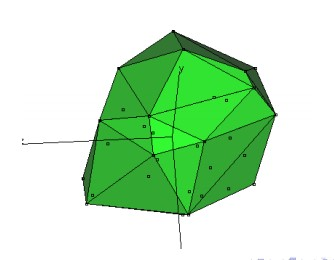
\includegraphics[width=0.6\linewidth]{simplex.jpg}%
    \end{center}


    % Если для расматриваемого ребра была уже найдена
    %
    % Хэш при неточных вычислениях.
    % Описать метод хеширования.
    % Перебор точек.
\end{frame}
\begin{frame}{Алгорим Джарвиса при необщем положении точек}
 % Грань -  Симплекс.ував
    % \vfill
    Проблемы расширения:
       \begin{itemize}
        \item  хранение выпуклой оболочки;
        \item  построение грани;
        \item  обход ребер.
        \end{itemize}
\end{frame}

\begin{frame}{Хранение выпуклой оболочки}
    % В результате появляются новые требования к хранению.

    % \begin{itemize}
    %     \item в несимплициальном случае недостаточно хранить только вершины, нужно хранить ребра, которые в свою очередь могут быть многомерными несимплициальными многогранниками;
    %     \item для дальнейшего использования разумно хранить список соседних граней;
    % \end{itemize}
    Требования к хранению:
    \begin{itemize}
        \item нужно хранить ребра, которые в свою очередь могут быть многомерными несимплициальными многогранниками;
        \item необходимо хранить список соседних граней;
        \item нужно хранить информацию о плоскости грани.
    \end{itemize}

    \pause
    \vfill

    % Решение:

    % Выпуклая оболочка $n$ - мерного пространства, это граф $F:=(V,E)$ , где $V$- непустое множество граней, а $E$ - множество пар соседних граней.

    Грань хранит:
    \begin{itemize}
        \item информацию плоскости: базис, уравнение плоскости;
        \item список соседних граней;
        \item структура грани:
        \begin{itemize}
            \item Если $R^d$ $(d>2)$, список ребер;
            \item Если $R^2$, список точек;
        \end{itemize}
        \end{itemize}

    %Для дальнейших вычислений необходимо хранить базис и уравнения плоскости. для каждой грани.
\end{frame}

% \begin{frame}{Хранение выпуклой оболочки}


%     % При $R^n$ $\left(n>2\right)$ грань $v$ --- выпуклая оболочка, граф $F'\in R^{n-1}$.

%     % При $R^2$ грань $v$ --- массив точек $P$.
% \end{frame}


\begin{frame}{Проблема построения грани}

    Проблемы построения:
    \begin{itemize}
        \item  априори невозможно указать, какие из точек, попавших в плоскость грани, являются ее вершинами;
        \item грани выпуклой оболочки могут содержать разное количество ребер.
    \end{itemize}
    % В плоскости грани могут содержаться точки, не являющиеся вершинами этой грани.
    \pause

    Решение --- уход в аффинное подпространство плоскости грани и построение в нем выпуклой оболочки роя точек, попавших в эту плоскость.

    Отдельное рассмотрение случая двумерного аффинного подпространства.

    \begin{minipage}{.4\textwidth}
        \centering
        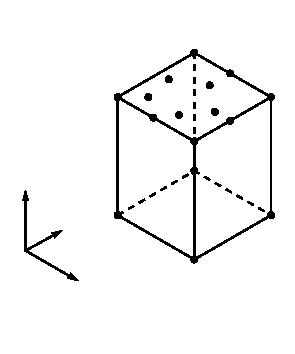
\includegraphics[width=\linewidth]{affine.pdf}
      \end{minipage}
      \begin{minipage}{.1\textwidth}
        \centering
        
\includegraphics[width=0.8\linewidth]{affine2.pdf}
      \end{minipage}
      \begin{minipage}{.4\textwidth}
        \centering
        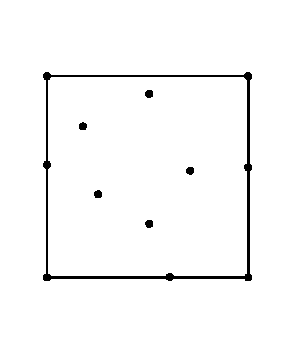
\includegraphics[width=\linewidth]{affine1.pdf}
      \end{minipage}

    % \vfill
    % \begin{center}
    %     \includegraphics[scale = 0.5]{./images/square.png}
    % \end{center}

\end{frame}
% Эти проблемы решаются уходом в афинное подпространстов грани. И построением выпуклой оболочки там.
% ДЛя этого нужно расширить алгоритм общего положения.
% После того как плоскость грани найдена, решая недоопределенную систему линейных уравлений находим нормаль плоскости.
% С помощью нормали находим все точки и переводим их координаты в базис плоскости.
%После этого ищем выпуклую оболочку набора точек.
\begin{frame}{Поиск первой грани}
    \vspace*{-5mm}

     \centerline{
        \only<1>{\input{./img/affinePoint.pdf_tex}}%
        \only<2>{\input{./img/affinePoint05.pdf_tex}}%
        \only<3>{\input{./img/affinePoint1.pdf_tex}}%
        \only<4>{\input{./img/affinePoint15.pdf_tex}}%
        \only<5>{\input{./img/affinePoint16.pdf_tex}}%
        \only<6>{\input{./img/affinePoint3.pdf_tex}}%
     }

    \only<1>{Найти плоскость грани \\}%
    \only<2>{Вычислить нормаль плоскости \\}%
    \only<3>{Найти точки и перевести в базис плоскости \\}%
    \only<4>{Построить выпуклую оболочку \\}%
    \only<5>{Найти и запомнить базисы ребер \\}%
    \only<6>{Заменить точки выпуклой оболочки на исходные и пересчитать базисные векторы ребер в координаты исходного пространства. Добавить грань в очередь на обработку. \\}%
\end{frame}

\begin{frame}{Переход через ребро}
    \vspace*{-5mm}

    % \only<1>{\input{./img/crossPN/crossPN.pdf_tex}}%
    \only<1>{\input{./img/crossPN/crossPN1.pdf_tex}}%
    \only<2>{\input{./img/crossPN/crossPN2.pdf_tex}}%
    \only<3>{\input{./img/crossPN/crossPN3.pdf_tex}}%
    \only<4>{\input{./img/crossPN/crossPN4.pdf_tex}}%
    \only<5>{\input{./img/crossPN/crossPN5.pdf_tex}}%
    % \only<6>{\input{./img/crossPN/crossPN6.pdf_tex}}%
    \only<6>{\input{./img/crossPN/crossPN7.pdf_tex}}%
    \only<7>{\input{./img/crossPN/crossPN8.pdf_tex}}%
    \only<8>{\input{./img/crossPN/crossPN9.pdf_tex}}%


    \only<1>{Если очередь граней на обработку пуста, остановить работу. Иначе взять грань из очереди. \\}%
    \only<2>{Взять очередное ребро обрабатываемой грани.\\}%
    \only<3>{Поочередно провести векторы к свободным точкам.\\}%
    \only<3>{Ортонормировать эти векторы на фоне базиса ребра (шаг процедуры Грама--Шмидта) \\}%
    \only<4>{Найти вектор, образующий максимальный угол с вектором грани. \\}%
    \only<5>{Плоскость грани найдена.\\}%
    \only<6>{Определить нормаль плоскости. Построить хэш плоскости грани и проверить, обработана ли она уже. Если обработана, запомнить информацию о соседстве граней и перейти к следующему ребру обрабатываемой грани. Иначе продолжить обработку новой грани. \\}%
    \only<7>{Найти точки, попавшие в плоскость грани. Если их $d+1$ штука, то грань симплициальная и не требует особой обработки. Иначе запустить рекурсивно алгоритм овыпукления в аффинном подпространстве.\\}%
    %  и выразить их в координатах пространства плоскости грани.
    \only<8>{Грань построена. Запомнить информацию о соседстве. Добавить в очередь на обработку.\\}%
\end{frame}
% \begin{frame}{Проблема построения грани}
%     % Как мы вытаскиваем объект исходного пространства.
%     % для этого необходимо доработать реализацию алгоритма построения выпуклой оболочки при общем положении.
%     % Напоследнем этапе постения у нас имеется базис плоскости, но нам еще известно сколько точек лежит на этой плоскости.
%     Порядок построения:
%     \begin{itemize}
%         \item найти плоскости грани;
%         \begin{itemize}
%             \item плоскость определяется нахождением симплицированной грани
%         \end{itemize}
%         \item найти уравнение плоскости;
%         \item определить точки, лежащие на плоскости;
%         \item перевести точки в базис плоскости;
%         \item найти выпуклую оболочку в координатах плоскости;
%         \item подменить точки выпуклой оболочки на исходные.
%     \end{itemize}

% \end{frame}


% \begin{frame}{Обход граней}
%     Обход происходит также как и в 2d
%     Порядок построения:
%     \begin{itemize}
%         \item поиск плоскости грани;
%         \item определение точек, лежащих на плоскости;
%         \item перевод точек в базис плоскости;
%         \item построение выпуклой оболочки в подпространстве;
%         \item подмена точек выпуклой оболочки на исходные.
%     \end{itemize}

% \end{frame}

% \begin{frame}{Алгоритм при необщем положении точек}

%     Вход --- Набор точек $R^d$ пространства;

%     Выход --- Выпуклая оболочка;
%     \begin{itemize}
%         \item Если $n = 2$ найти выпуклую оболочку на плоскости;
%         \item Если количество точек равно $n+1$ построить симплекс;
%         \item Найти первую грань и добавить ее в очередь;
%         \item Пока очередь не пуста, брать грань и производить переход для каждого ребра.
%         \item Если грань новая добавляются в очередь, иначе добавить в соседние.
%     \end{itemize}

% \end{frame}


% \begin{frame}{Поиск первой грани}

%     \begin{itemize}
%         \item Найти первую грань:
%         \begin{itemize}
%             \item найти плоскость начальной грани;
%             \item найти точки и перевести их в базис плоскости;
%             \item рекурсивно найти выпуклую оболочку;
%         \end{itemize}
%         \item добавить грань в очередь на рассмотрение;
%     \end{itemize}

% \end{frame}

% \begin{frame}{Построение выпуклой оболочки}

%     Повторять пока очередь не пустая:
%         \begin{itemize}
%         \item взять из очереди грань;
%         \item для каждого ребра грани повторить:
%         \begin{itemize}
%             \item найти плоскость соседней грани;
%             \item найти точки и перевести их в базис плоскости;
%             \item рекурсивно найти выпуклую оболочку;
%             \item если грань не обрабатывалась, добавить ее в очередь;
%             \item иначе обозначить соседство граней;
%         \end{itemize}
%     \end{itemize}

% \end{frame}


%
%

\begin{frame}{Результат}

    % Для обхога всех граней был использован обход в ширину.
    % При обработки грани, для всех ее ребер находятся соседние грани.
    % Если грань новая то ее добавляют в очередь
    % Для хранения информации о найденных гранях была использована хэш таблица.
    Сложность --- $O\big((hn)^{d-1}\big)$,\\
    где $h$ --- количество ребер, $n$ --- количество точек, $d$~---~размерность.
    \vfill
    \begin{center}
        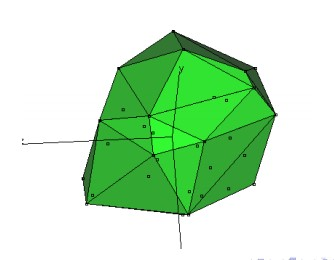
\includegraphics[width=0.6\linewidth]{simplex.jpg}%
    \end{center}


    % Если для расматриваемого ребра была уже найдена
    %
    % Хэш при неточных вычислениях.
    % Описать метод хеширования.
    % Перебор точек.
\end{frame}


\begin{frame}{Тестовая реализация}

Платформа -.Net Core. \\
Язык - C\#.

\end{frame}

\begin{frame}{Пример работы алгоритма}
    \begin{center}
        \includegraphics[width=\linewidth]{regular.jpg}
    \end{center}
\end{frame}

% \begin{frame}{Пример работы алгоритма}
%     Массив точек четырехмерном пространства.
% \end{frame}
% \begin{frame}{Пример работы алгоритма}
%     Проекции граней.
%     \begin{center}
%         \includegraphics[width=0.5\linewidth]{./images/regular.jpg}
%     \end{center}
% \end{frame}


\end{document}
